\documentclass[aspectratio=169,10pt]{beamer}

\usepackage{amsmath,amssymb,mathtools}
\usepackage{booktabs,tabularx,array}
\usepackage{graphicx}
\usepackage{tikz}
\usetikzlibrary{arrows.meta,positioning,shapes.geometric}
\usepackage{listings}
\usepackage{xcolor}

\usetheme{Madrid}
\usecolortheme{default}
\definecolor{CourseNavy}{HTML}{17365D}
\definecolor{CourseTeal}{HTML}{168C8C}
\definecolor{CourseOrange}{HTML}{D97706}
\definecolor{CourseLight}{HTML}{EEF4F8}
\definecolor{CourseRed}{HTML}{B42318}
\setbeamercolor{structure}{fg=CourseNavy}
\setbeamercolor{palette primary}{bg=CourseNavy,fg=white}
\setbeamercolor{palette secondary}{bg=CourseTeal,fg=white}
\setbeamercolor{palette tertiary}{bg=CourseNavy!85,fg=white}
\setbeamercolor{frametitle}{bg=CourseNavy,fg=white}
\setbeamercolor{block title}{bg=CourseNavy!12,fg=CourseNavy}
\setbeamercolor{block body}{bg=CourseLight!70,fg=black}
\setbeamercolor{alerted text}{fg=CourseRed}
\setbeamertemplate{navigation symbols}{}
\setbeamertemplate{itemize item}{\color{CourseTeal}$\blacktriangleright$}
\setbeamertemplate{itemize subitem}{\color{CourseOrange}$\bullet$}
\setbeamertemplate{section in toc}[sections numbered]

\newcommand{\E}{\mathbb{E}}
\newcommand{\Var}{\operatorname{Var}}
\newcommand{\dd}{\,\mathrm{d}}
\newcommand{\Normal}{\mathcal{N}}
\newcommand{\code}[1]{\texttt{#1}}
\newcommand{\good}[1]{\textcolor{CourseTeal}{#1}}

\lstset{
  language=Python,
  basicstyle=\ttfamily\scriptsize,
  keywordstyle=\color{CourseNavy}\bfseries,
  commentstyle=\color{CourseTeal!80!black},
  stringstyle=\color{CourseOrange!90!black},
  showstringspaces=false,
  frame=single,
  rulecolor=\color{CourseNavy!25},
  backgroundcolor=\color{CourseLight!55},
  columns=fullflexible,
  keepspaces=true
}

\title[Financial SDEs: Numerical Simulation]{Numerical Simulation of Financial Stochastic Differential Equations}
\subtitle{From Euler--Maruyama to Nested-Grid Verification}
\author[Group Presentation]{%
  \begin{tabular}{c}
    \textbf{Group Members}\\[0.25em]
    Member 1: \underline{\hspace{2.7cm}}\quad Student ID: \underline{\hspace{2.3cm}}\\[0.12em]
    Member 2: \underline{\hspace{2.7cm}}\quad Student ID: \underline{\hspace{2.3cm}}\\[0.12em]
    Member 3: \underline{\hspace{2.7cm}}\quad Student ID: \underline{\hspace{2.3cm}}\\[0.12em]
    Member 4: \underline{\hspace{2.7cm}}\quad Student ID: \underline{\hspace{2.3cm}}\\[0.12em]
    Member 5: \underline{\hspace{2.7cm}}\quad Student ID: \underline{\hspace{2.3cm}}
  \end{tabular}%
}
\institute{Numerical Partial Differential Equations}
\date{September 2026}

\AtBeginSection[]{
  \begin{frame}[plain]
    \vfill
    \centering
    {\usebeamerfont{title}\color{CourseNavy}\insertsectionnumber.\ \insertsectionhead\par}
    \vspace{0.8em}
    {\color{CourseTeal}\rule{0.56\linewidth}{1.2pt}}
    \vfill
  \end{frame}
}

\begin{document}

\begin{frame}
  \titlepage
\end{frame}

\begin{frame}{Purpose of the Presentation}
  \begin{block}{Intended audience}
    Students familiar with elementary probability and the explicit Euler method,
    but with no prior background in stochastic calculus or mathematical finance.
  \end{block}
  By the end of the presentation, the audience should be able to explain:
  \begin{enumerate}
    \item how an SDE is discretised on a time grid;
    \item why Monte Carlo averages estimate expectations;
    \item how Euler--Maruyama and Milstein differ;
    \item what strong and weak convergence measure;
    \item how to validate a solver when no exact solution is available;
    \item what the numerical evidence does and does not establish.
  \end{enumerate}
\end{frame}

\begin{frame}{The Numerical Workflow}
  \centering
  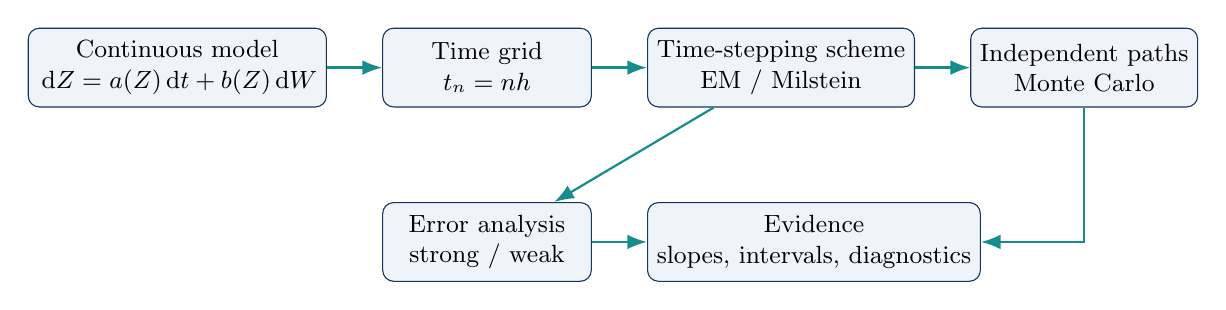
\begin{tikzpicture}[
    node distance=7mm and 7mm,
    box/.style={draw=CourseNavy,rounded corners,fill=CourseLight,
      minimum width=2.65cm,minimum height=1.0cm,align=center,font=\small},
    arr/.style={-{Latex[length=2.5mm]},thick,draw=CourseTeal}
  ]
    \node[box] (model) {Continuous model\\$\dd Z=a(Z)\dd t+b(Z)\dd W$};
    \node[box,right=of model] (grid) {Time grid\\$t_n=nh$};
    \node[box,right=of grid] (scheme) {Time-stepping scheme\\EM / Milstein};
    \node[box,right=of scheme] (mc) {Independent paths\\Monte Carlo};
    \node[box,below=12mm of grid] (error) {Error analysis\\strong / weak};
    \node[box,right=of error] (evidence) {Evidence\\slopes, intervals, diagnostics};
    \draw[arr] (model)--(grid);
    \draw[arr] (grid)--(scheme);
    \draw[arr] (scheme)--(mc);
    \draw[arr] (mc)|-(evidence);
    \draw[arr] (scheme)--(error);
    \draw[arr] (error)--(evidence);
  \end{tikzpicture}
  \vspace{1em}
  \begin{alertblock}{Central numerical-analysis question}
    A simulation is credible only when the discretisation, error reduction,
    statistical uncertainty, and reproducibility are all made explicit.
  \end{alertblock}
\end{frame}

\begin{frame}{Connection with Numerical PDEs}
  For the diffusion
  \[
    \dd S_t=a(S_t)\dd t+b(S_t)\dd W_t,
  \]
  define
  \[
    u(t,s)=\E\!\left[\varphi(S_T)\mid S_t=s\right].
  \]
  Under standard assumptions, $u$ satisfies the backward Kolmogorov equation
  \[
    u_t+a(s)u_s+\frac12 b(s)^2u_{ss}=0,
    \qquad u(T,s)=\varphi(s).
  \]
  \begin{block}{Two numerical routes}
    \begin{itemize}
      \item discretise the PDE in $(t,s)$;
      \item discretise sample paths in time and approximate the expectation by Monte Carlo.
    \end{itemize}
  \end{block}
  This coursework uses the second route while retaining the central themes of
  \alert{discretisation, convergence, stable computation, and error quantification}.
\end{frame}

\begin{frame}{Two Models, Two Numerical Roles}
  \begin{tabularx}{\textwidth}{>{\bfseries}p{2.3cm}XX}
    \toprule
      & Model 1: GBM benchmark & Model 2: non-affine coupled model \\
    \midrule
    Purpose & exact solution for verification & realistic test without a closed form \\
    Methods & exact update, EM, Milstein & log-variable Euler--Maruyama \\
    Main outputs & strong and weak errors, moments & nested-grid differences and nonlinear observables \\
    Reference & exact terminal value on the same path & a much finer numerical grid \\
    Main difficulty & separating pathwise and expectation errors & controlling reference-solution error \\
    \bottomrule
  \end{tabularx}
  \vspace{0.7em}

  \centering
  \good{The exact benchmark validates the implementation before it is used in a model without an exact solution.}
\end{frame}

\begin{frame}{Structure}
  \tableofcontents[hideallsubsections]
\end{frame}

\section{From the Euler Method to Stochastic Time Stepping}

\begin{frame}{Review: Explicit Euler for an ODE}
  Consider
  \[
    \frac{\dd y}{\dd t}=f(y),\qquad y(0)=y_0,
  \]
  on the grid
  \[
    0=t_0<t_1<\cdots<t_N=T,\qquad h=\frac{T}{N}.
  \]
  Freezing the slope over one time step gives
  \[
    y(t_{n+1})-y(t_n)\approx f(y_n)h,
    \qquad \boxed{y_{n+1}=y_n+f(y_n)h}.
  \]
  \begin{block}{Key idea}
    The continuous evolution is replaced by many short steps. A smaller $h$
    usually improves the approximation, at greater computational cost.
  \end{block}
\end{frame}

\begin{frame}{An SDE Adds a Random Increment}
  A scalar stochastic differential equation is
  \[
    \boxed{\dd Z_t=a(Z_t)\dd t+b(Z_t)\dd W_t}.
  \]
  \begin{itemize}
    \item $a(Z_t)\dd t$: drift, analogous to deterministic ODE motion;
    \item $b(Z_t)\dd W_t$: diffusion, representing random fluctuations;
    \item $W_t$: Brownian motion, whose paths are not differentiable.
  \end{itemize}
  Over one interval,
  \[
    Z_{t_{n+1}}-Z_{t_n}
    =\int_{t_n}^{t_{n+1}}a(Z_t)\dd t
     +\int_{t_n}^{t_{n+1}}b(Z_t)\dd W_t.
  \]
  Freezing both coefficients at the left endpoint produces the stochastic Euler method.
\end{frame}

\begin{frame}{Brownian Increments in the Code}
  Brownian increments satisfy
  \[
    \Delta W_n=W_{t_{n+1}}-W_{t_n}\sim\Normal(0,h),
    \qquad \Delta W_n=\sqrt{h}\,Z_n,\quad Z_n\sim\Normal(0,1).
  \]
  \begin{columns}[T]
    \column{0.48\textwidth}
    \begin{block}{Mean}
      \[
        \E[\Delta W_n]=0.
      \]
      Positive and negative disturbances cancel on average.
    \end{block}
    \column{0.48\textwidth}
    \begin{block}{Scale}
      \[
        \operatorname{SD}(\Delta W_n)=\sqrt h.
      \]
      The random increment is $O(\sqrt h)$ rather than $O(h)$.
    \end{block}
  \end{columns}
  \begin{alertblock}{Common implementation error}
    Using $hZ_n$ suppresses the stochastic term too rapidly and changes the limiting model.
  \end{alertblock}
\end{frame}

\begin{frame}{Euler--Maruyama}
  Freeze both coefficients during one step:
  \[
    \int_{t_n}^{t_{n+1}}a(Z_t)\dd t\approx a(Z_n)h,\qquad
    \int_{t_n}^{t_{n+1}}b(Z_t)\dd W_t\approx b(Z_n)\Delta W_n.
  \]
  The Euler--Maruyama (EM) method is
  \[
    \boxed{Z_{n+1}=Z_n+a(Z_n)h+b(Z_n)\Delta W_n}.
  \]
  \begin{itemize}
    \item It is explicit: only the known state $Z_n$ is used.
    \item One sequence of increments generates one approximate path.
    \item Many paths are required to estimate expectations and uncertainty.
  \end{itemize}
\end{frame}

\begin{frame}{Monte Carlo Estimation}
  To estimate $\E[X]$, generate independent samples $X^{(1)},\ldots,X^{(M)}$:
  \[
    \widehat m_M=\frac1M\sum_{i=1}^M X^{(i)}.
  \]
  The law of large numbers gives $\widehat m_M\to\E[X]$, while
  \[
    \operatorname{SE}(\widehat m_M)\approx\frac{s_X}{\sqrt M}.
  \]
  An approximate $95\%$ confidence interval is
  \[
    \boxed{\widehat m_M\pm1.96\frac{s_X}{\sqrt M}}.
  \]
  \begin{alertblock}{Cost implication}
    Halving the Monte Carlo standard error requires approximately four times as many paths.
  \end{alertblock}
\end{frame}

\begin{frame}{Two Contributions to the Total Error}
  \[
    \underbrace{\widehat Q_{h,M}-Q}_{\text{total error}}
    =
    \underbrace{\bigl(\E[Q_h]-Q\bigr)}_{\text{time-discretisation bias}}
    +
    \underbrace{\bigl(\widehat Q_{h,M}-\E[Q_h]\bigr)}_{\text{sampling noise}}.
  \]
  Typical magnitudes are
  \[
    |\text{bias}|\approx Ch^p,
    \qquad
    |\text{sampling error}|\approx C_M M^{-1/2}.
  \]
  \begin{block}{Experimental design principle}
    To measure a time-convergence rate, sampling noise must remain below the
    discretisation error over the fitted grid range.
  \end{block}
\end{frame}

\begin{frame}{Why Stochastic Taylor Expansions Need a Correction}
  For smooth $f$, It\^o's formula is
  \[
    \dd f(Z_t)
      =f'(Z_t)\dd Z_t+\frac12f''(Z_t)b(Z_t)^2\dd t.
  \]
  The final term is absent from the ordinary chain rule. It appears because
  \[
    \Delta W=O(\sqrt h)
    \quad\Longrightarrow\quad
    (\Delta W)^2=O(h).
  \]
  \begin{block}{Sufficient intuition for this coursework}
    Some second-order random terms are as large as the deterministic drift term
    and therefore cannot be discarded.
  \end{block}
\end{frame}

\begin{frame}{Milstein: One Additional Random Second-Order Term}
  For $\dd Z=a(Z)\dd t+b(Z)\dd W$, the scalar Milstein method is
  \[
    \boxed{
    Z_{n+1}=Z_n+a(Z_n)h+b(Z_n)\Delta W_n
    +\frac12 b(Z_n)b'(Z_n)\bigl((\Delta W_n)^2-h\bigr)}.
  \]
  \begin{itemize}
    \item The first three terms are exactly Euler--Maruyama.
    \item The correction has zero mean because $\E[(\Delta W)^2]=h$.
    \item It improves pathwise local accuracy.
    \item In scalar problems, it typically raises the strong order from $1/2$ to $1$.
  \end{itemize}
\end{frame}

\begin{frame}{Coupling Coarse and Fine Paths}
  If one coarse step contains $q$ fine steps, define
  \[
    \Delta W^{\mathrm{coarse}}_k
      =\sum_{j=1}^{q}\Delta W^{\mathrm{fine}}_{kq+j}.
  \]
  Then
  \[
    \Delta W^{\mathrm{coarse}}_k\sim\Normal(0,qh_{\mathrm{fine}}).
  \]
  \begin{columns}[T]
    \column{0.48\textwidth}
      \begin{block}{Coupled comparison}
        Coarse and fine solutions use the same Brownian path; their difference
        primarily measures discretisation error.
      \end{block}
    \column{0.48\textwidth}
      \begin{block}{Independent comparison}
        Separate random inputs mainly measure the difference between two random paths.
      \end{block}
  \end{columns}
\end{frame}

\begin{frame}{Strong and Weak Errors}
  \begin{columns}[T]
    \column{0.48\textwidth}
    \begin{block}{Strong error: are paths close?}
      \[
        e_{\rm strong}(h)=\E|Z_T^h-Z_T|.
      \]
      Both values must share the same Brownian path.
    \end{block}
    \column{0.48\textwidth}
    \begin{block}{Weak error: are statistics close?}
      \[
        e_{\rm weak}(h)=
        \left|\E\varphi(Z_T^h)-\E\varphi(Z_T)\right|.
      \]
      Only the expectation of a chosen observable is compared.
    \end{block}
  \end{columns}
  \begin{alertblock}{They are not interchangeable}
    A method may be inaccurate path by path while estimating a particular expectation accurately.
  \end{alertblock}
\end{frame}

\begin{frame}{Reading a Convergence Order}
  If $e(h)\approx Ch^p$, then
  \[
    \log e\approx \log C+p\log h.
  \]
  Hence a log--log slope estimates the order $p$.
  \begin{center}
    \begin{tabular}{ccc}
      \toprule
      Order & factor when $h$ is halved & two successive halvings \\
      \midrule
      $p=1/2$ & $2^{-1/2}\approx0.707$ & error approximately halves \\
      $p=1$   & $2^{-1}=0.5$          & error is approximately quartered \\
      \bottomrule
    \end{tabular}
  \end{center}
  \alert{A slope must be interpreted together with its fitting range,
  uncertainty, and reference-solution error.}
\end{frame}

\section{Model 1: Verification against an Exact Solution}

\begin{frame}{Geometric Brownian Motion as a Test Equation}
  \[
    \boxed{\dd S_t=\mu S_t\dd t+\sigma S_t\dd W_t},
    \qquad S_0=100,\ \mu=0.05,\ \sigma=0.30,\ T=1.
  \]
  \begin{itemize}
    \item Drift and diffusion are proportional to the current state.
    \item Financially, it is a simple price model; numerically, it is a solvable test equation.
    \item Its exact solution permits direct error measurement.
    \item The exact state remains positive, providing an additional diagnostic.
  \end{itemize}
  \begin{block}{Why begin with this model?}
    A solver should reproduce known benchmark behaviour before it is used
    on a model without an exact solution.
  \end{block}
\end{frame}

\begin{frame}{Deriving the Exact GBM Solution}
  Apply It\^o's formula to $f(S)=\log S$:
  \[
    \dd\log S_t
    =\frac{1}{S_t}\dd S_t-\frac12\frac{1}{S_t^2}(\sigma S_t)^2\dd t
    =\left(\mu-\frac12\sigma^2\right)\dd t+\sigma\dd W_t.
  \]
  Therefore
  \[
    \boxed{S_t=S_0\exp\!\left[
      \left(\mu-\frac12\sigma^2\right)t+\sigma W_t
    \right]}.
  \]
  \begin{alertblock}{Interpretation}
    The term $-\sigma^2/2$ follows from the stochastic chain rule;
    it is not an additional financial assumption.
  \end{alertblock}
\end{frame}

\begin{frame}{Exact Moments as Distribution-Level Checks}
  \[
    \E[S_T]=S_0e^{\mu T},\qquad
    \Var(S_T)=S_0^2e^{2\mu T}\bigl(e^{\sigma^2T}-1\bigr).
  \]
  For the reported parameters,
  \[
    \E[S_T]=105.1271,\qquad \Var(S_T)=1040.7868.
  \]
  Exact terminal sampling produced
  \[
    \widehat{\E}[S_T]=105.1987,\qquad
    \widehat{\Var}(S_T)=1045.0120.
  \]
  These differences are consistent with Monte Carlo sampling variation.
\end{frame}

\begin{frame}{Three One-Step Updates for GBM}
  Let $\Delta W_n\sim\Normal(0,h)$.
  \begin{align*}
    \text{Exact:}\quad
    S_{n+1}&=S_n\exp\!\left[
      \left(\mu-\tfrac12\sigma^2\right)h+\sigma\Delta W_n\right],\\
    \text{Euler--Maruyama:}\quad
    S_{n+1}&=S_n\left(1+\mu h+\sigma\Delta W_n\right),\\
    \text{Milstein:}\quad
    S_{n+1}&=S_n\left[1+\mu h+\sigma\Delta W_n
      +\tfrac12\sigma^2\bigl((\Delta W_n)^2-h\bigr)\right].
  \end{align*}
  \begin{block}{Fair comparison}
    All three updates reuse the same increments, so terminal differences
    reflect numerical error rather than different random inputs.
  \end{block}
\end{frame}

\begin{frame}[fragile]{Core GBM Implementation}
\begin{lstlisting}
h = T / N
dW = np.sqrt(h) * rng.standard_normal((M, N))

S_em  = np.full(M, S0)
S_mil = np.full(M, S0)
for n in range(N):
    dw = dW[:, n]
    S_em *= 1.0 + mu*h + sigma*dw
    S_mil *= (1.0 + mu*h + sigma*dw
              + 0.5*sigma**2*(dw**2 - h))

W_T = dW.sum(axis=1)
S_exact = S0*np.exp((mu - 0.5*sigma**2)*T + sigma*W_T)
\end{lstlisting}
  \vspace{-0.4em}
  \begin{itemize}
    \item The arrays advance $M$ paths simultaneously.
    \item The exact value uses the sum of the same increments.
  \end{itemize}
\end{frame}

\begin{frame}{GBM Experimental Protocol}
  \begin{itemize}
    \item $T=1$, grid sizes $N=2^k$, and time step $h=T/N$.
    \item A fixed number of paths and a recorded random seed are used.
    \item Strong error:
      $\widehat e=M^{-1}\sum_i|S_{T,i}^{h}-S_{T,i}^{\rm exact}|$.
    \item Its standard error is computed from the pathwise absolute differences.
    \item Weak mean error is evaluated analytically whenever possible.
    \item Log--log regression is applied over a stated asymptotic range.
  \end{itemize}
  \begin{alertblock}{Role of the seed}
    A fixed seed does not improve accuracy. It permits exact reproduction of the sample.
  \end{alertblock}
\end{frame}

\begin{frame}{GBM Strong-Convergence Results}
  \centering
  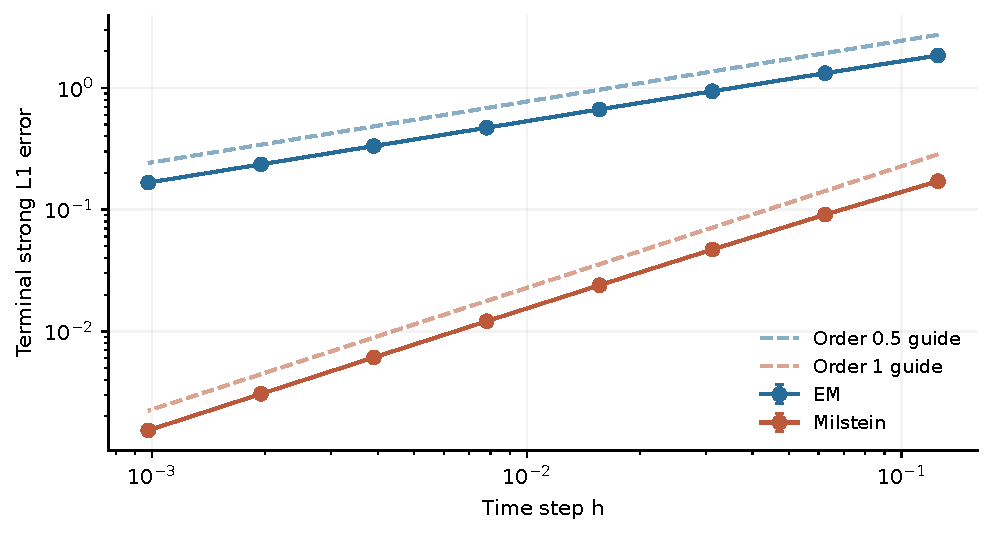
\includegraphics[width=0.88\textwidth,height=0.72\textheight,keepaspectratio]{assets_en/gbm_strong.pdf}

  \vspace{-0.4em}
  \small Fitted slopes: EM $0.500$; Milstein $0.991$.
\end{frame}

\begin{frame}{Interpreting the Strong-Error Plot}
  \begin{columns}[T]
    \column{0.52\textwidth}
    \begin{tabular}{lcc}
      \toprule
      Method & $N=64$ & $N=1024$ \\
      \midrule
      EM & $0.66641$ & $0.16658$ \\
      Milstein & $0.02391$ & $0.00153$ \\
      \bottomrule
    \end{tabular}
    \column{0.44\textwidth}
    \begin{itemize}
      \item Increasing $N$ by $16$ reduces $h$ by $16$.
      \item EM error decreases by approximately $4=16^{1/2}$.
      \item Milstein error decreases by approximately $15.6\approx16^1$.
    \end{itemize}
  \end{columns}
  \vspace{0.5em}
  \begin{block}{Conclusion}
    The data agree with strong order $1/2$ for EM and strong order $1$ for Milstein.
  \end{block}
\end{frame}

\begin{frame}{Individual Challenge: Before and After}
  \begin{columns}[T]
    \column{0.49\textwidth}
      \centering
      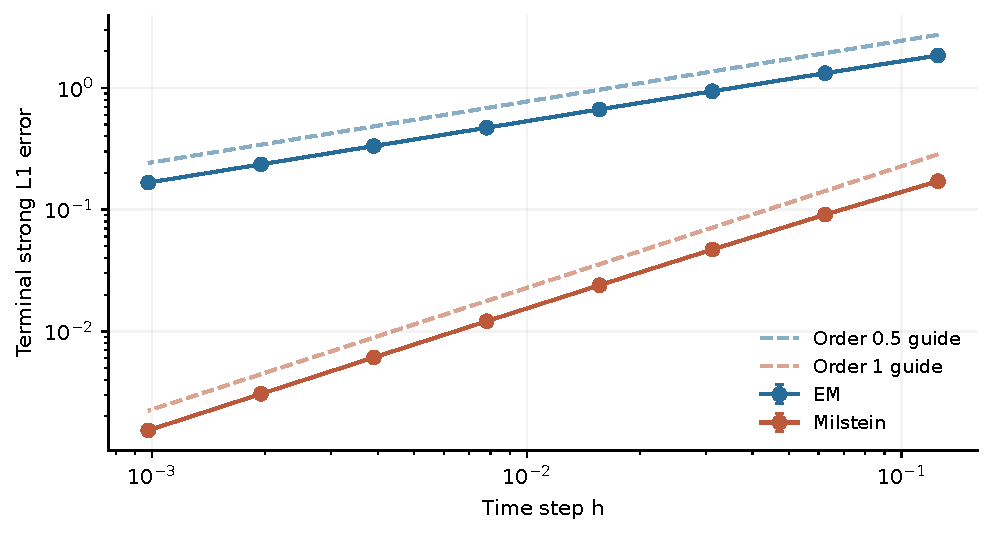
\includegraphics[width=\linewidth,height=0.54\textheight,keepaspectratio]{assets_en/gbm_strong_before.pdf}

      \small\textbf{Before:} error curves alone do not quantify slope stability.
    \column{0.49\textwidth}
      \centering
      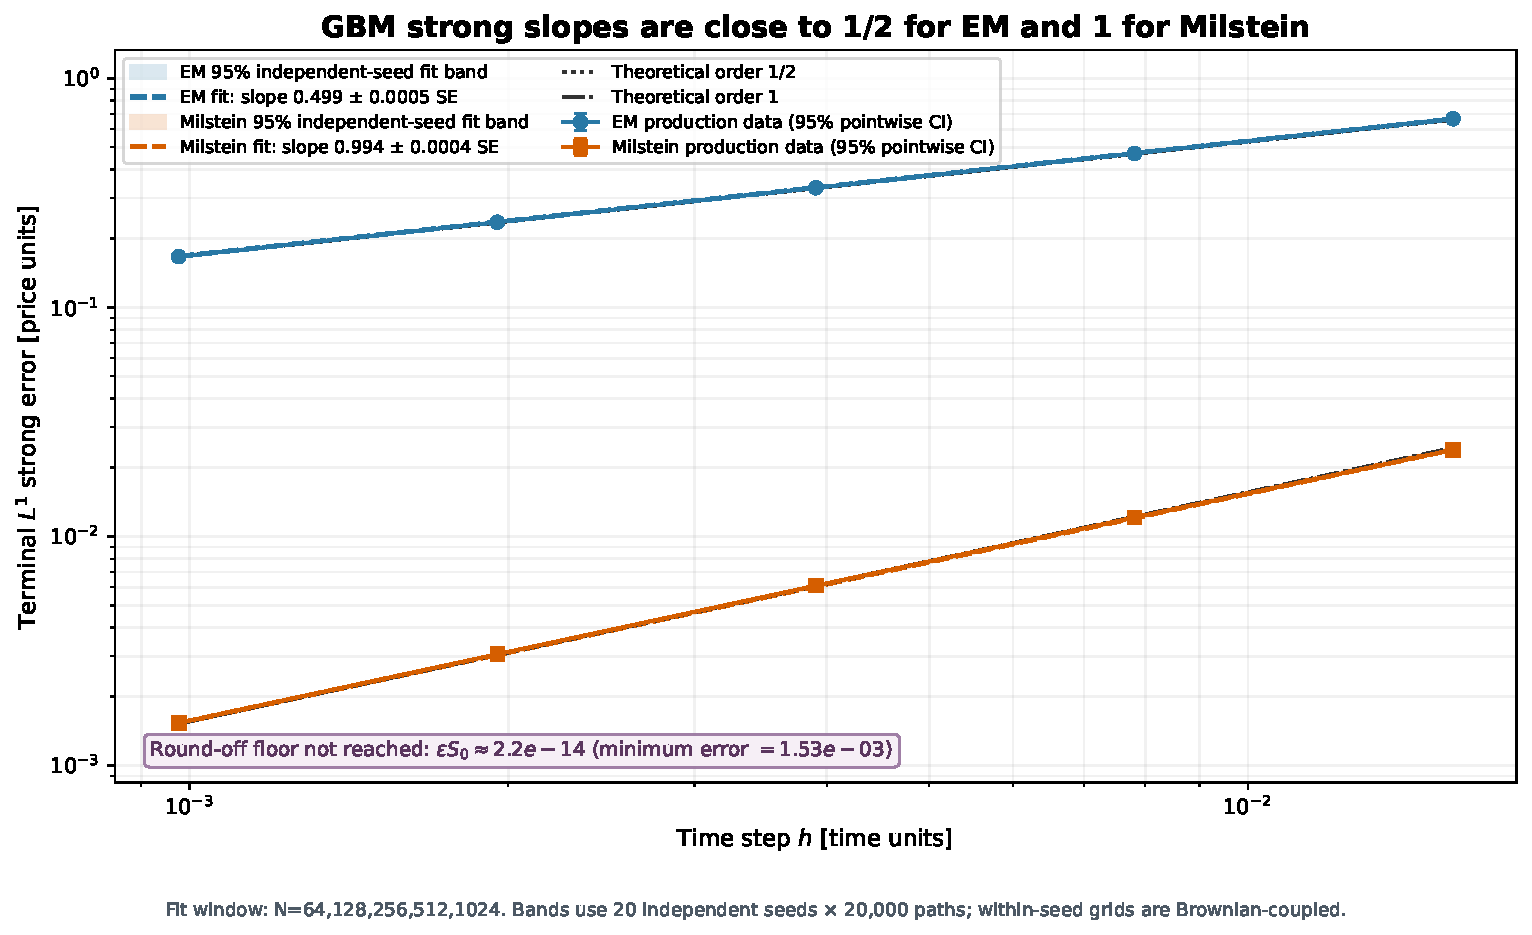
\includegraphics[width=\linewidth,height=0.54\textheight,keepaspectratio]{assets_en/gbm_strong_after.pdf}

      \small\textbf{After:} repeated-run error bars, theory guides, and fitted slopes.
  \end{columns}
  \vspace{0.2em}
  \centering\footnotesize
  The revision turns a qualitative visual claim into quantitative, reproducible evidence.
\end{frame}

\begin{frame}{Analytic Weak Mean Error}
  Euler--Maruyama satisfies
  \[
    \E[S_{n+1}^{\rm EM}\mid S_n^{\rm EM}]
      =S_n^{\rm EM}(1+\mu h),
  \]
  and hence
  \[
    \E[S_N^{\rm EM}]=S_0(1+\mu h)^N,\qquad N=T/h.
  \]
  The Milstein correction has zero expectation, so both methods have the same mean.
  Comparing with $S_0e^{\mu T}$ gives
  \[
    \boxed{e_{\rm weak}(h)=
      \left|S_0(1+\mu h)^{T/h}-S_0e^{\mu T}\right|=O(h)}.
  \]
\end{frame}

\begin{frame}{GBM Weak-Convergence Results}
  \centering
  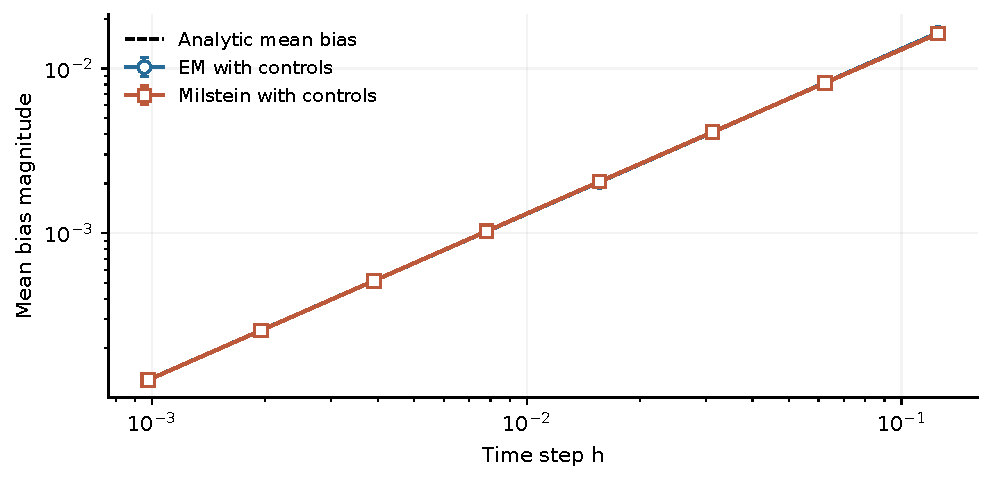
\includegraphics[width=0.88\textwidth,height=0.70\textheight,keepaspectratio]{assets_en/gbm_weak.pdf}

  \vspace{-0.5em}
  \small EM slope $0.999$ and Milstein slope $1.000$.
  The curves coincide because both methods have the same analytic mean bias.
\end{frame}

\begin{frame}{Why Better Paths Do Not Improve This Mean}
  \begin{itemize}
    \item Milstein improves the agreement of each numerical path with the exact path.
    \item Its additional correction has zero mean.
    \item For $\varphi(S)=S$, EM and Milstein therefore have identical weak errors.
    \item A different nonlinear observable may produce a different comparison.
  \end{itemize}
  \begin{alertblock}{Orders must be associated with an error criterion}
    Milstein has higher \emph{strong} order in this benchmark.
    This does not imply higher weak order for every observable.
  \end{alertblock}
\end{frame}

\begin{frame}{Distribution Check}
  \centering
  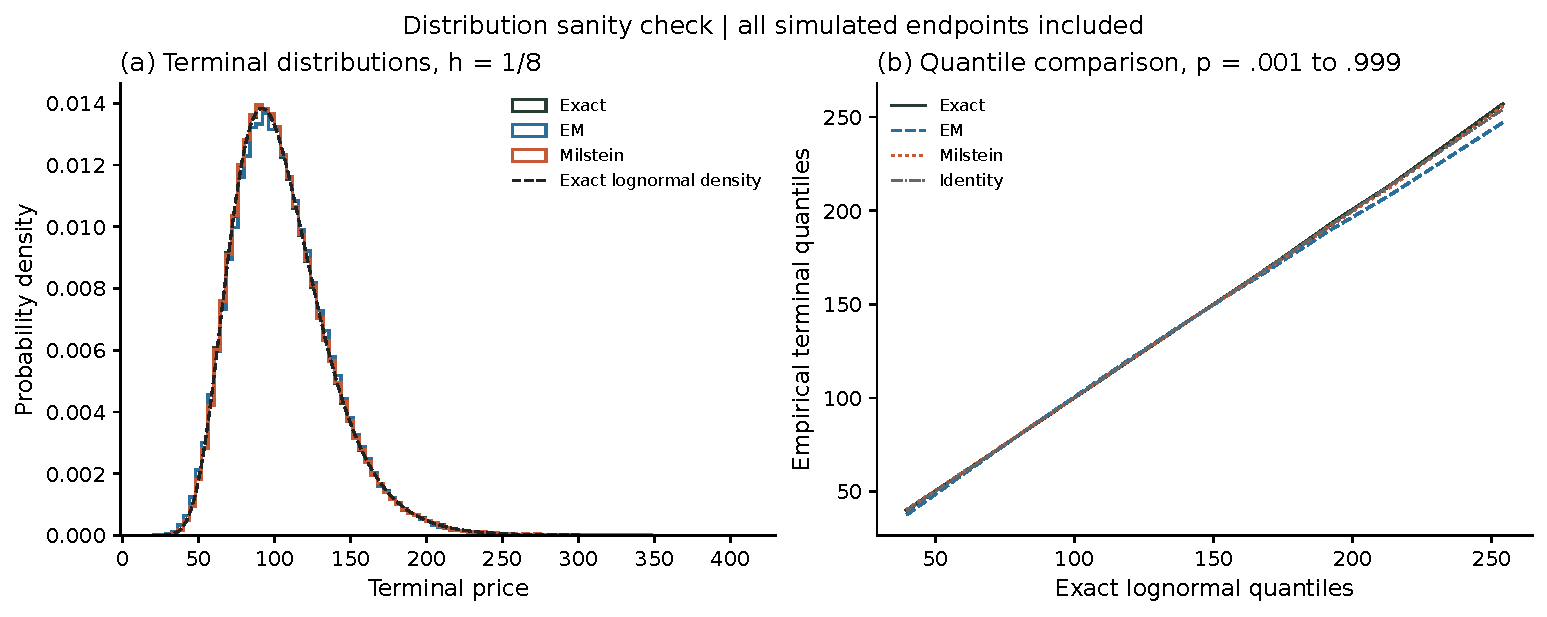
\includegraphics[width=0.88\textwidth,height=0.70\textheight,keepaspectratio]{assets_en/gbm_distribution.pdf}

  \vspace{-0.5em}
  \small The histogram should agree with the exact lognormal density, while
  sample moments should agree within plausible Monte Carlo uncertainty.
\end{frame}

\begin{frame}{Positivity Check}
  The exact solution is strictly positive. A discrete method need not preserve this property.
  \begin{center}
    \begin{tabular}{lcc}
      \toprule
      Terminal-value method & negative values / paths & empirical frequency \\
      \midrule
      Exact update & $0/160000$ & $0.000\%$ \\
      Euler--Maruyama & $0/160000$ & $0.000\%$ \\
      Milstein & $0/160000$ & $0.000\%$ \\
      \bottomrule
    \end{tabular}
  \end{center}
  \begin{alertblock}{Scope}
    This is an empirical terminal-time frequency for the reported parameters and grids.
    It is not a proof of positivity preservation for all cases.
  \end{alertblock}
\end{frame}

\begin{frame}{What the GBM Benchmark Established}
  \begin{enumerate}
    \item Brownian increments use the correct $\sqrt h$ scaling.
    \item Exact and numerical values are coupled through the same path.
    \item EM and Milstein reproduce the expected strong orders.
    \item Both methods have first-order weak mean error for a precise analytic reason.
    \item Moment, distribution, and positivity checks support the implementation.
  \end{enumerate}
  \begin{block}{Next step}
    Replace the unavailable exact solution by a controlled fine-grid numerical reference.
  \end{block}
\end{frame}

\section{Model 2: Nested-Grid Verification without an Exact Solution}

\begin{frame}{A Non-Affine Model with State-Dependent Volatility}
  Let $S_t=e^{X_t}$ and consider
  \begin{align*}
    \dd X_t&=\left(\mu-\frac12g(Y_t)^2\right)\dd t+g(Y_t)\dd W_t^{(1)},\\
    \dd Y_t&=\kappa(\theta-Y_t)\dd t
      +\xi\sqrt{1+Y_t^2}\dd W_t^{(2)},\\
    g(y)&=0.1+\frac{0.4}{1+e^{-y}},
    \qquad \operatorname{Corr}(\dd W^{(1)},\dd W^{(2)})=\rho.
  \end{align*}
  \begin{itemize}
    \item $Y_t$ changes the noise amplitude of $X_t$.
    \item The coefficient functions are non-affine.
    \item No directly usable exact terminal solution is available.
  \end{itemize}
\end{frame}

\begin{frame}{Parameter Set}
  \begin{center}
    \begin{tabular}{clc}
      \toprule
      Parameter & Numerical role & Value \\
      \midrule
      $S_0,Y_0$ & initial conditions & $100,0$ \\
      $\mu$ & mean growth component of $X$ & $0.05$ \\
      $\kappa,\theta$ & mean-reversion rate and centre for $Y$ & $2,-0.2$ \\
      $\xi$ & noise scale in $Y$ & $0.6$ \\
      $\rho$ & correlation between random drivers & $-0.7$ \\
      $T$ & terminal time & $1$ \\
      \bottomrule
    \end{tabular}
  \end{center}
  \begin{block}{Minimal financial interpretation}
    Treat $S$ as a positive state and $Y$ as a second state controlling its
    instantaneous random fluctuation. No pricing theory is required.
  \end{block}
\end{frame}

\begin{frame}{Generating Correlated Brownian Increments}
  Generate independent $Z_1,Z_2\sim\Normal(0,1)$ and define
  \[
    \Delta W_1=\sqrt h Z_1,\qquad
    \Delta W_2=\sqrt h\left(\rho Z_1+\sqrt{1-\rho^2}Z_2\right).
  \]
  Then
  \[
    \Var(\Delta W_1)=\Var(\Delta W_2)=h,\qquad
    \operatorname{Corr}(\Delta W_1,\Delta W_2)=\rho.
  \]
  \begin{alertblock}{Required diagnostic}
    The observed sample correlation was $-0.699675$, compared with the target $-0.7$.
  \end{alertblock}
\end{frame}

\begin{frame}{Why Discretise $X=\log S$?}
  A direct update of $S$ may become negative after a sufficiently large negative
  random increment. Updating $X$ and transforming back gives
  \[
    S_n=e^{X_n}>0
  \]
  whenever $X_n$ remains finite.
  \begin{block}{A structure-aware numerical choice}
    The variable transformation uses analytic structure to preserve a state constraint,
    in the same spirit as structure-aware PDE discretisations.
  \end{block}
\end{frame}

\begin{frame}{Synchronous Euler--Maruyama Update}
  Both components use the old state $Y_n$:
  \begin{align*}
    X_{n+1}&=X_n+\left(\mu-\frac12g(Y_n)^2\right)h
      +g(Y_n)\Delta W_{1,n},\\
    Y_{n+1}&=Y_n+\kappa(\theta-Y_n)h
      +\xi\sqrt{1+Y_n^2}\Delta W_{2,n},\\
    S_{n+1}&=e^{X_{n+1}}.
  \end{align*}
  \begin{alertblock}{Meaning of synchronous}
    $X_{n+1}$ and $Y_{n+1}$ must both use $Y_n$. Updating $Y$ first and using
    the new value in the $X$ step would implement a different scheme.
  \end{alertblock}
\end{frame}

\begin{frame}[fragile]{Implementation Details}
\begin{lstlisting}
def g(y):
    # stable sigmoid avoids exponential overflow
    return 0.1 + 0.4 * expit(y)

for n in range(N):
    y_old = y.copy()
    gy = g(y_old)
    x += (mu - 0.5*gy**2)*h + gy*dW1[:, n]
    y += kappa*(theta - y_old)*h \
         + xi*np.sqrt(1.0 + y_old**2)*dW2[:, n]

assert np.isfinite(x).all() and np.isfinite(y).all()
s = np.exp(x)
\end{lstlisting}
  \vspace{-0.4em}
  \small Recorded diagnostics include finite-state checks, increment variances,
  correlation, and the number of non-positive prices.
\end{frame}

\begin{frame}{An Exact Structural Property of the Discrete Mean}
  Conditional on $\mathcal F_n$, $g(Y_n)$ is known. Since
  \[
    \E[e^{a\Delta W}]=e^{a^2h/2},
  \]
  \begin{align*}
    \E[S_{n+1}\mid\mathcal F_n]
      &=S_ne^{(\mu-\frac12g_n^2)h}\E[e^{g_n\Delta W_{1,n}}]\\
      &=S_ne^{\mu h}.
  \end{align*}
  Hence
  \[
    \boxed{\E[S_N]=S_0e^{\mu T}\quad\text{for every step size }h.}
  \]
  \begin{alertblock}{Consequence for weak testing}
    The observable $\varphi(S)=S$ has zero time-discretisation bias and cannot
    test whether the terminal distribution is approximated correctly.
  \end{alertblock}
\end{frame}

\begin{frame}{Why Use a Call Payoff as the Nontrivial Observable?}
  Choose
  \[
    \varphi(S)=(S-K)^+=\max(S-K,0),\qquad K=100.
  \]
  \begin{itemize}
    \item It is nonlinear, so $\E[\varphi(S)]$ is not determined by $\E[S]$.
    \item Equal means do not imply equal payoff expectations.
    \item It detects changes in the shape and upper tail of the terminal distribution.
    \item Its kink at $S=K$ makes the weak rate more difficult to resolve numerically.
  \end{itemize}
  \begin{block}{Reason for the choice}
    Once the linear mean is exact by construction, a distribution-sensitive
    observable is required. Detailed financial interpretation is unnecessary.
  \end{block}
\end{frame}

\begin{frame}{Nested Fine-Grid Reference}
  Use the same finest Brownian increments to construct
  \[
    S_T^{N}\quad\text{and}\quad S_T^{N_{\rm ref}},
    \qquad N_{\rm ref}\gg N.
  \]
  The coupled strong difference is
  \[
    \widehat D_N=\frac1M\sum_{i=1}^M
      \left|S_{T,i}^{N}-S_{T,i}^{N_{\rm ref}}\right|.
  \]
  For a weak observable, use the paired difference
  \[
    \widehat B_N=\frac1M\sum_{i=1}^M
      \left[\varphi(S_{T,i}^{N})-\varphi(S_{T,i}^{N_{\rm ref}})\right].
  \]
  \begin{alertblock}{Precise terminology}
    These are differences relative to a numerical reference, not known exact errors.
    Reference-grid sensitivity must therefore be investigated.
  \end{alertblock}
\end{frame}

\begin{frame}{Nested-Grid Experimental Design}
  \begin{center}
    \begin{tabular}{ll}
      \toprule
      Component & Setting \\
      \midrule
      Coarse grids & $N=8,16,32,64,128,256$ \\
      Main reference grid & $N_{\rm ref}=8192$ \\
      Sensitivity references & $2048,4096,8192$ \\
      Number of paths & $M=100000$ \\
      Coupling & all grids aggregate the same finest increments \\
      Strong quantity & $\E|S_T^N-S_T^{N_{\rm ref}}|$ \\
      Weak quantities & mean difference and paired call-payoff difference \\
      \bottomrule
    \end{tabular}
  \end{center}
  The strong-rate fit uses $N=8,16,32,64$ to limit curvature caused by the
  finite reference grid at the finest coarse levels.
\end{frame}

\begin{frame}{Non-Affine Strong-Difference Results}
  \centering
  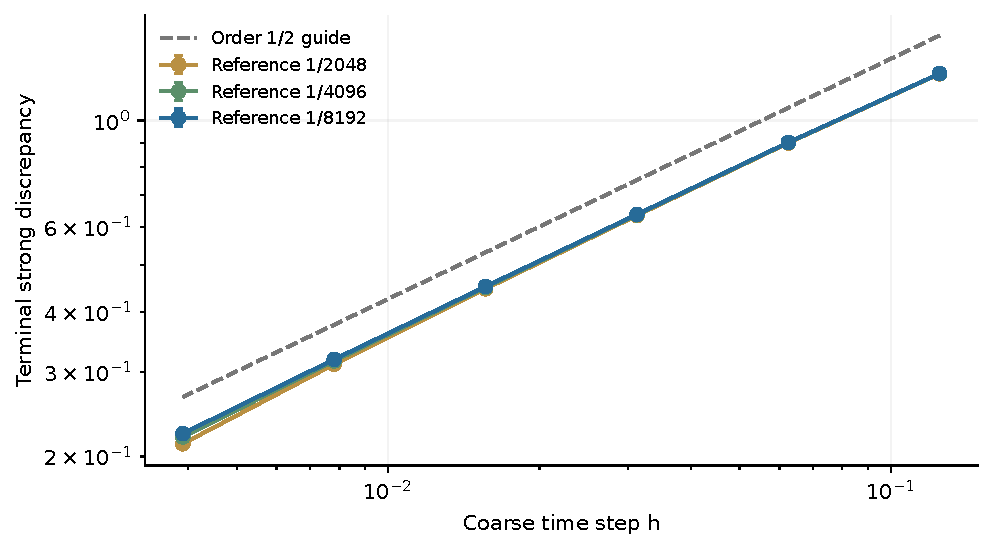
\includegraphics[width=0.88\textwidth,height=0.71\textheight,keepaspectratio]{assets_en/nonaffine_strong.pdf}

  \vspace{-0.5em}
  \small The fitted slope relative to $N_{\rm ref}=8192$ is $0.491$,
  consistent with the typical strong order $1/2$ of Euler--Maruyama.
\end{frame}

\begin{frame}{Reference-Grid Sensitivity}
  Hold the fitted coarse grids $N=8,16,32,64$ fixed:
  \begin{center}
    \begin{tabular}{ccl}
      \toprule
      $N_{\rm ref}$ & fitted slope & interpretation \\
      \midrule
      $2048$ & $0.496$ & coarser reference, similar slope \\
      $4096$ & $0.493$ & close to the finer result \\
      $8192$ & $0.491$ & main reported reference \\
      \bottomrule
    \end{tabular}
  \end{center}
  \begin{block}{Supported conclusion}
    The approximately half-order slope is stable under these reference choices.
    Their agreement is numerical evidence, not an exact error bound.
  \end{block}
\end{frame}

\begin{frame}{The Reference Also Has Discretisation Error}
  Differences between successive reference levels are
  \[
    \E|S_T^{2048}-S_T^{4096}|\approx0.05679,\qquad
    \E|S_T^{4096}-S_T^{8192}|\approx0.04016.
  \]
  Their ratio is
  \[
    \frac{0.04016}{0.05679}\approx0.707\approx2^{-1/2}.
  \]
  \begin{itemize}
    \item The reference levels themselves show half-order reduction.
    \item The $8192$-step solution is not exact.
    \item It is sufficiently fine to reveal a stable slope for $N=8$ to $64$.
  \end{itemize}
\end{frame}

\begin{frame}{Non-Affine Weak Differences}
  \centering
  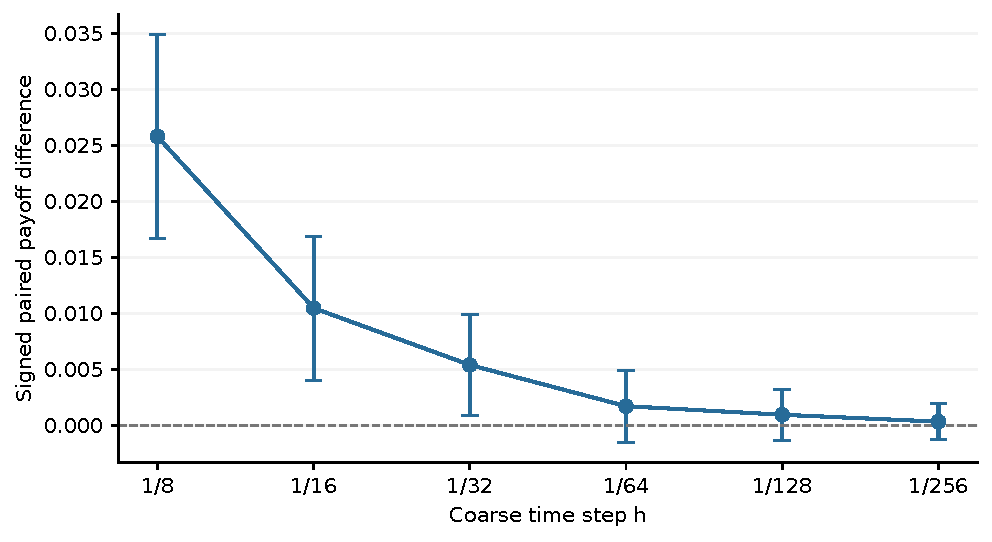
\includegraphics[width=0.88\textwidth,height=0.71\textheight,keepaspectratio]{assets_en/nonaffine_weak.pdf}

  \vspace{-0.5em}
  \small Coarse-grid payoff differences are statistically resolved.
  At finer grids, confidence intervals include zero and sampling noise is
  comparable with the discretisation difference.
\end{frame}

\begin{frame}{Why No Reliable Weak Order Is Reported}
  \begin{itemize}
    \item For $N=8,16,32$, paired-payoff confidence intervals exclude zero.
    \item For $N=64,128,256$, the intervals include zero.
    \item At fine levels, the sign and magnitude are sensitive to sampling noise.
    \item A log--log fit would mistake noise for an asymptotic convergence law.
    \item The payoff kink also makes the asymptotic regime harder to resolve.
  \end{itemize}
  \begin{alertblock}{Correct interpretation}
    Weak differences decrease, but the available sample budget is insufficient
    for a credible weak-order estimate. This limits the evidence; it does not
    demonstrate failure of the numerical scheme.
  \end{alertblock}
\end{frame}

\begin{frame}{Sample-Size Experiment}
  Fix $N=64$ and $N_{\rm ref}=8192$:
  \begin{center}
    \begin{tabular}{rrrr}
      \toprule
      $M$ & paired difference & standard error & $95\%$ interval \\
      \midrule
      $10{,}000$  & $0.009045$ & $0.005149$ & $[-0.001048,\ 0.019137]$ \\
      $40{,}000$  & $0.004942$ & $0.002592$ & $[-0.000139,\ 0.010022]$ \\
      $100{,}000$ & $0.001722$ & $0.001633$ & $[-0.001479,\ 0.004923]$ \\
      \bottomrule
    \end{tabular}
  \end{center}
  \begin{itemize}
    \item The standard error decreases approximately as $M^{-1/2}$.
    \item All three intervals still include zero.
    \item A larger budget or variance reduction is needed for rate estimation.
  \end{itemize}
\end{frame}

\begin{frame}{Mean and Implementation Diagnostics}
  The exact discrete-mean identity predicts
  \[
    \E[S_T^N]=100e^{0.05}=105.1271.
  \]
  The finest simulation produced
  \[
    \widehat{\E}[S_T]=105.08796,
    \qquad 95\%\text{ CI }[104.89962,105.27629],
  \]
  which contains the theoretical value. The associated payoff estimate was
  \[
    14.53804,\qquad 95\%\text{ CI }[14.40515,14.67093].
  \]
  \begin{block}{Different roles}
    The mean checks the implementation; the nonlinear payoff probes distributional weak error.
  \end{block}
\end{frame}

\begin{frame}{Numerical Diagnostic Checklist}
  \begin{center}
    \begin{tabularx}{\textwidth}{>{\bfseries}p{3.5cm}X}
      \toprule
      Diagnostic & Observation \\
      \midrule
      increment variances & consistent with $1/8192\approx1.221\times10^{-4}$ \\
      increment correlation & $-0.699675$, target $-0.7$ \\
      finite states & all reported $X$, $Y$, and $S$ values were finite \\
      positivity & $S=e^X$ remained positive \\
      exact mean identity & theoretical mean lies inside the empirical interval \\
      reference sensitivity & three reference grids give similar strong slopes \\
      \bottomrule
    \end{tabularx}
  \end{center}
  A visually convincing convergence plot does not replace these checks.
\end{frame}

\section{Evaluation, Reproducibility, and Conclusions}

\begin{frame}{What the Coursework Requires}
  \begin{tabularx}{\textwidth}{>{\bfseries}p{3.1cm}XX}
    \toprule
    Component & Required task & Evidence reported here \\
    \midrule
    GBM strong convergence & compare EM and Milstein with theory & slopes $0.500$ and $0.991$ \\
    GBM weak behaviour & choose and explain an observable & analytic first-order mean bias \\
    distribution / positivity & quantitative checks & moments, histogram, negative frequency \\
    non-affine strong study & nested grids and sensitivity & stable half-order trend \\
    non-affine weak study & intervals and justified conclusion & trend visible; rate unresolved \\
    reproducibility & commands, seed, environment, Git & traceable code and outputs \\
    \bottomrule
  \end{tabularx}
  \vspace{0.6em}
  A weak order need not be forced from unresolved data. The requirement is a
  sound experiment and an evidence-based interpretation.
\end{frame}

\begin{frame}{Code Structure Mirrors the Mathematics}
  \begin{enumerate}
    \item \textbf{Parameters:} initial data, coefficients, $T$, grids, paths, seed.
    \item \textbf{Random increments:} finest-grid normal samples and correlation transform.
    \item \textbf{Solvers:} EM, Milstein, and log-variable EM.
    \item \textbf{Coupling:} aggregation of fine increments for each coarse grid.
    \item \textbf{Statistics:} means, standard errors, intervals, fitted slopes.
    \item \textbf{Outputs:} tables, figures, data, and run metadata.
  \end{enumerate}
  \begin{block}{Practical benefit}
    An anomalous plot can be traced through statistic, path, increment, and parameter layers.
  \end{block}
\end{frame}

\begin{frame}{A Minimal Reproducibility Chain}
  \centering
  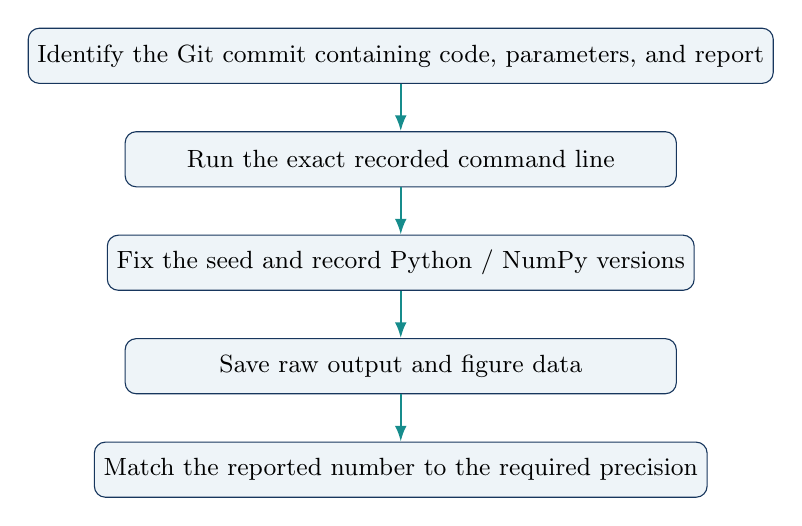
\begin{tikzpicture}[
    node distance=6mm,
    box/.style={draw=CourseNavy,rounded corners,fill=CourseLight,
      minimum width=7.0cm,minimum height=7mm,align=center,font=\small},
    arr/.style={-{Latex[length=2mm]},thick,draw=CourseTeal}
  ]
    \node[box] (c) {Identify the Git commit containing code, parameters, and report};
    \node[box,below=of c] (cmd) {Run the exact recorded command line};
    \node[box,below=of cmd] (env) {Fix the seed and record Python / NumPy versions};
    \node[box,below=of env] (out) {Save raw output and figure data};
    \node[box,below=of out] (match) {Match the reported number to the required precision};
    \draw[arr] (c)--(cmd);
    \draw[arr] (cmd)--(env);
    \draw[arr] (env)--(out);
    \draw[arr] (out)--(match);
  \end{tikzpicture}
  \vspace{0.6em}

  If a script and report disagree, correct the report or identify the version difference.
\end{frame}

\begin{frame}{Eight Common Failure Modes}
  \begin{enumerate}
    \item using $hZ$ instead of $\sqrt h Z$ for Brownian increments;
    \item comparing independent paths when measuring strong error;
    \item confusing sample standard deviation with standard error;
    \item refining $h$ without checking the Monte Carlo noise floor;
    \item updating $Y$ before using it in the synchronous $X$ update;
    \item describing a finite fine-grid solution as exact;
    \item fitting a weak rate to sign-unstable differences whose intervals include zero;
    \item reporting a slope without the fitting range, uncertainty, and diagnostics.
  \end{enumerate}
\end{frame}

\begin{frame}{How to Read a Convergence Plot Critically}
  Ask the following questions in order:
  \begin{enumerate}
    \item Is the horizontal axis $h$, $N$, or computational cost?
    \item Is the vertical quantity an exact error or a reference difference?
    \item Are coarse and fine solutions driven by the same random input?
    \item Do error bars show standard deviation, standard error, or confidence intervals?
    \item Which points are used in the slope fit, and why?
    \item Do the finest points reach a noise or reference-error floor?
    \item Is the conclusion stable under changes in sample size or reference grid?
  \end{enumerate}
  \begin{alertblock}{Practical rule}
    Identify what the vertical axis measures before assessing linearity or reading a slope.
  \end{alertblock}
\end{frame}

\begin{frame}{Main Conclusions}
  \begin{enumerate}
    \item EM and Milstein show GBM strong orders close to $1/2$ and $1$.
    \item For the terminal mean, both methods share the same first-order weak bias.
    \item Nested-grid experiments support half-order strong convergence in the non-affine model.
    \item The non-affine discretisation preserves the mean exactly, so a nonlinear
      payoff is needed to detect distributional weak error.
    \item The present path budget supports a decreasing weak-difference trend,
      but not a credible weak-order estimate.
    \item Confidence intervals, reference sensitivity, and diagnostics are as important as slopes.
  \end{enumerate}
\end{frame}

\begin{frame}{Possible Extensions}
  \begin{enumerate}
    \item Increase paired samples or use a control variate for payoff differences.
    \item Balance $h$ and $M$ under a fixed computational budget.
    \item Refine the reference grid and quantify its systematic contribution.
    \item Report uncertainty in the fitted convergence slope.
    \item Compare Monte Carlo with a finite-difference solution of the associated
      backward PDE for a simplified one-dimensional model.
  \end{enumerate}
  \begin{block}{Scope}
    These are natural extensions. The present coursework should first explain
    its existing evidence and limitations clearly.
  \end{block}
\end{frame}

\begin{frame}[plain]
  \vfill
  \centering
  {\Huge\color{CourseNavy}Thank you}

  \vspace{1em}
  {\Large Questions?}

  \vspace{2em}
  \begin{minipage}{0.78\textwidth}
    \centering
    \color{CourseTeal}
    Starting from the Euler method, three additions were essential:
    \textbf{normal increments, repeated sampling, and quantified uncertainty}.
  \end{minipage}
  \vfill
\end{frame}

\appendix
\section{Backup Derivations}

\begin{frame}{Backup: Why Is the GBM Mean Bias First Order?}
  Let $N=T/h$. Since
  \[
    \log(1+\mu h)=\mu h-\frac12\mu^2h^2+O(h^3),
  \]
  \begin{align*}
    (1+\mu h)^{T/h}
      &=\exp\!\left[\frac{T}{h}\log(1+\mu h)\right]\\
      &=\exp\!\left[\mu T-\frac12\mu^2Th+O(h^2)\right]\\
      &=e^{\mu T}\left(1-\frac12\mu^2Th+O(h^2)\right).
  \end{align*}
  Therefore
  \[
    S_0(1+\mu h)^{T/h}-S_0e^{\mu T}=O(h).
  \]
\end{frame}

\begin{frame}{Backup: Why Pairing Reduces Noise}
  Compare
  \begin{align*}
    \text{independent:}\quad
      &\widehat{\E}[\varphi(S^N)]-\widehat{\E}[\varphi(S^{\rm ref})],\\
    \text{paired:}\quad
      &\frac1M\sum_i\left[\varphi(S_i^N)-\varphi(S_i^{\rm ref})\right].
  \end{align*}
  For a paired difference,
  \[
    \Var(A-B)=\Var(A)+\Var(B)-2\operatorname{Cov}(A,B).
  \]
  A shared Brownian path makes $A$ and $B$ strongly positively correlated,
  so common path fluctuations cancel in the difference.
\end{frame}

\begin{frame}{Backup: Standard Error and Sample Size}
  For paired samples $D_1,\ldots,D_M$,
  \[
    \bar D=\frac1M\sum_iD_i,\qquad
    s_D^2=\frac1{M-1}\sum_i(D_i-\bar D)^2,\qquad
    \operatorname{SE}(\bar D)=\frac{s_D}{\sqrt M}.
  \]
  To reduce the standard error from $\varepsilon_1$ to $\varepsilon_2$,
  \[
    M_2\approx M_1\left(\frac{\varepsilon_1}{\varepsilon_2}\right)^2.
  \]
  Reducing it by a factor of five requires approximately twenty-five times as many paths.
\end{frame}

\begin{frame}{Backup: Terminology}
  \begin{tabularx}{\textwidth}{>{\bfseries}p{3.0cm}X}
    \toprule
    Term & Meaning in this coursework \\
    \midrule
    drift & deterministic mean change per unit time \\
    diffusion & amplitude of the random fluctuation \\
    Brownian increment & normal variable with mean $0$ and variance $h$ \\
    path & a complete sequence $Z_0,Z_1,\ldots,Z_N$ \\
    observable & a terminal function $\varphi(Z_T)$ \\
    strong convergence & numerical and exact values approach on the same path \\
    weak convergence & expectations of an observable approach \\
    nested grid & coarse increments are sums of shared fine increments \\
    numerical reference & a fine-grid approximation used for an unknown exact solution \\
    \bottomrule
  \end{tabularx}
\end{frame}

\begin{frame}{References and Project Files}
  \begin{thebibliography}{9}
    \bibitem{problem-pack}
    Course Problem Pack, Direction 4: Financial SDEs, pp.~6--7.

    \bibitem{higham}
    D.~J. Higham,
    \newblock An Algorithmic Introduction to Numerical Simulation of Stochastic Differential Equations,
    \newblock \emph{SIAM Review}, 43(3), 2001.

    \bibitem{kloeden-platen}
    P.~E. Kloeden and E.~Platen,
    \newblock \emph{Numerical Solution of Stochastic Differential Equations},
    \newblock Springer, 1992.
  \end{thebibliography}
  \vspace{0.3em}
  \small Project scripts: \code{gbm.py}, \code{nonaffine.py};
  undergraduate report: \code{undergraduate\_revision/}.
\end{frame}

\end{document}
